% Every number in this paper is copied from vision/RESULTS.md (run numbers given in comments).
% Compiles with pdflatex on its own (no venue style file). For submission, move the body
% into the venue's official template (e.g. on Overleaf) and anonymise as required.
\documentclass[10pt,twocolumn,letterpaper]{article}
\usepackage[margin=0.75in,columnsep=0.3in]{geometry}
\usepackage{times}
\usepackage{graphicx}
\usepackage{booktabs}
\usepackage{amsmath}
\usepackage{multirow}
\usepackage[hidelinks]{hyperref}
\usepackage[capitalise,noabbrev]{cleveref}
\usepackage{xcolor}
\usepackage{caption}
\captionsetup{font=small,labelfont=bf}
\setlength{\tabcolsep}{4pt}

\title{\Large\bf How Much Is a Real Fall Worth?\\Real, Synthetic and Staged Training Data for Video Fall Detection,\\Tested on Two Real-World Sources}
\author{Anonymous submission}
\date{}

\begin{document}
\maketitle

\begin{abstract}
Video fall detectors are commonly trained and evaluated on falls staged by actors in a laboratory, where they score near perfectly. We ask which training data actually prepares a detector for real falls. We build \textbf{FallOrNot}, a real-world test set from the OOPS!\ dataset of in-the-wild accident videos, sampled independently of any model and labelled for whether a person falls, so that \emph{other accidents} act as false-alarm negatives. Using frozen CLIP and VideoMAE features with linear probes, and end-to-end fine-tuned VideoMAE, we compare staged (UR Fall), synthetic (OmniFall OF-Syn) and real (OOPS!) training data, and test on FallOrNot and on an independent real-world source, HMDB51. Staged-trained probes that score 1.00 in-domain reach 0.76 AUROC on FallOrNot. On FallOrNot, 131 real training falls lift the best probe to 0.90, and about 30 real falls outperform 2,136 synthetic ones, whose benefit plateaus near 0.82. On HMDB51, however, the ranking flips: synthetic training is best and real training is no better than staged. The flip holds for fine-tuned models across three seeds. Mixing synthetic and real data is the only recipe that stays near the top on both test sets. A pre-registered test of whether fine-tuning beats frozen probes on both test sets was not met. A second annotator agreed moderately with the first ($\kappa=0.50$); re-grading with their labels preserves the main findings but weakens the in-domain real-over-synthetic advantage. Conclusions about training data drawn from a single real-world benchmark do not generalise; fall detectors should be evaluated on several.
\end{abstract}

%=====================================================================
\section{Introduction}
Falls are the second-leading cause of unintentional injury death worldwide, and about 71\% of fall deaths occur in people aged 60 or older~\cite{who_falls}; long periods on the floor after a fall are associated with worse outcomes~\cite{fleming2008}. Camera-based fall detection promises automatic alerts without wearables, and published detectors often report near-perfect accuracy. Most of that evidence comes from staged datasets in which young actors fall onto mattresses in front of fixed cameras~\cite{kwolek2014,charfi2013}.

Real falls are different: they are sudden, partly occluded, filmed from arbitrary viewpoints, and embedded among other abrupt events such as collisions, dropped objects and people catching themselves. OmniFall~\cite{omnifall} recently showed a large drop from staged to in-the-wild falls on fall-containing OOPS!~\cite{epstein2020oops} videos, and argued that synthetic training videos generalise better than staged ones. This leaves practical questions open for anyone building a detector: \emph{how much real data is needed, is real data worth more than synthetic data, does the answer change with the test set, and how often do detectors raise alarms for accidents that are not falls?}

\paragraph{Contributions.}
\begin{enumerate}\setlength\itemsep{1pt}
\item \textbf{FallOrNot}, a real-world test set sampled from \emph{all} annotated OOPS!\ accidents independently of any model, so that non-fall accidents are hard false-alarm negatives, plus pre-accident clips of ordinary activity.
\item A controlled comparison of \textbf{staged, synthetic and real training data} with identical encoders, probes and clips, including an equal-budget curve and a learning curve over the number of real falls.
\item Evidence that \textbf{rankings flip between real-world test sets}: real data wins on FallOrNot, synthetic data wins on an independent source (HMDB51), for both frozen probes and fine-tuned models; synthetic + real is the robust choice.
\item A \textbf{pre-registered} fine-tuning test (not met), a second-annotator agreement study, and a re-analysis with the second annotator's labels.
\end{enumerate}

%=====================================================================
\section{Related work}
\paragraph{Staged fall datasets.} UR Fall~\cite{kwolek2014} records 30 falls from a side and a ceiling camera and 40 activities of daily living; Le2i~\cite{charfi2013} and the Multiple Cameras Fall Dataset~\cite{auvinet_mcfd} are other widely used staged sets. Detectors evaluated on such data routinely approach ceiling performance.

\paragraph{Simulated vs.\ real falls.} For wearable accelerometers, algorithms tuned on simulated falls lose accuracy on real-world falls~\cite{bagala2012}, and the FARSEEING repository collects body-worn sensor signals from real falls~\cite{klenk2016}. We study the analogous question for video.

\paragraph{In-the-wild video.} OOPS!~\cite{epstein2020oops} contains about 20k web videos of unintentional actions with annotated transition times. \textbf{OmniFall}~\cite{omnifall}, the closest work, unifies eight staged datasets, adds 12k synthetic videos (OF-Syn) and an in-the-wild test set of 818 fall-containing OOPS!\ videos (OF-ItW), shows a large staged-to-wild drop, finds synthetic training better than staged, and reports an upper-bound model trained with in-the-wild data. We do not claim to be first to show the staged-to-wild gap. Our work differs in (i) negatives drawn from all accidents by a model-independent sample, (ii) the question of how much real data is needed and whether it beats synthetic data at equal budget, and (iii) testing every conclusion on a second, independent real-world source.

\paragraph{Encoders.} We use CLIP~\cite{radford2021clip} through OpenCLIP~\cite{openclip} with DataComp weights~\cite{gadre2023datacomp}, and VideoMAE~\cite{tong2022videomae} fine-tuned on Kinetics-400~\cite{kay2017kinetics}.

%=====================================================================
\section{The FallOrNot test set}
\paragraph{Source and clips.} We use the 10,961 OOPS!\ videos whose transition time $t$ was found by at least two annotators (median used). Each video yields an \emph{event} clip $[t-1, t+1]$\,s and, when $t\ge3.5$\,s, a \emph{pre-event} clip $[t-3.5, t-1.5]$\,s of ordinary activity. Every clip, in every dataset in this paper, is 2\,s long and sampled at 16 frames.

\paragraph{Model-independent test sample.} A video enters the test sample if the MD5 hash of its name falls below a fixed threshold (about 600 videos; 422 with usable clips). Selection depends on no model, so the benchmark cannot favour any detector. Clips were labelled in a fixed random order, so any labelled prefix is itself a random sample.

\paragraph{Labels.} Following the WHO definition, a fall is an event in which a person inadvertently comes to rest on the ground, floor or another lower level~\cite{who_falls}. The annotator answered \emph{fall}, \emph{not a fall} (including other accidents, near-falls and animals) or \emph{unsure} (excluded). Positives are event clips labelled \emph{fall}; negatives are event clips labelled \emph{not a fall} (hard negatives) and the pre-event clips of labelled test videos (easy negatives).

\paragraph{Size.} 165 test videos are labelled (255 clips, 102 falls). A separate training pool, the 3,000 event clips with the highest zero-shot CLIP fall score (never overlapping the test sample), provides 268 labelled real training clips (131 falls). The pool is model-selected and used only for training.

\paragraph{Second annotator.} An independent second annotator labelled 100 of the test videos without seeing the first annotator's answers. On the 98 clips both labelled \emph{fall} or \emph{not a fall}, raw agreement was 0.796 and Cohen's $\kappa=0.498$ [0.297, 0.678] (moderate). Disagreements were asymmetric: in 16 of 20 cases the second annotator saw a fall where the first did not (\cref{sec:annotator}).

%=====================================================================
\section{Experimental setup}
\paragraph{Training data.} \emph{Staged}: UR Fall~\cite{kwolek2014}; fall clips are centred on the frames labelled ``falling'', negatives are pre-fall clips and 2\,s windows (1\,s stride) over the activity videos; 316 clips, 60 falls (30 falls $\times$ 2 cameras). \emph{Synthetic}: OmniFall OF-Syn~\cite{omnifall}; one clip per video, centred on the fall segment for all 2,136 videos containing a fall and on the longest segment for 3,000 hash-sampled videos without one. \emph{Real}: the 268 labelled OOPS!\ training clips.

\paragraph{External real-world test: HMDB51.} HMDB51~\cite{kuehne2011hmdb} is independent of OOPS!. We use all 100 human-labelled \texttt{fall\_floor} clips and 20 hash-sampled clips from each of the other 50 classes. A hard subset, fixed in advance, keeps falls and whole-body or ground-contact actions (cartwheel, flic-flac, somersault, handstand, dive, jump, sit, sit-up, push-up, stand, climb; 320 clips). Clips are covered by 2\,s windows every 1\,s and scored by their maximum window. Nothing is trained on HMDB51.

\paragraph{Representations and detectors.} \emph{CLIP appearance}: mean of 8 L2-normalised CLIP ViT-L/14 frame embeddings. \emph{CLIP temporal}: [mean, last-third minus first-third, mean absolute frame-to-frame change]. \emph{VideoMAE}: pooled VideoMAE-B (Kinetics-400) embedding of 16 frames. \emph{CLIP + VideoMAE}: concatenation of the last two. Detectors are zero-shot CLIP (fall vs.\ non-fall prompt margin, prompts fixed in advance) and L2-regularised logistic regression on standardised features ($C=0.1$, class-balanced).

\paragraph{Fine-tuning.} VideoMAE-B fine-tuned end to end with hyper-parameters fixed before any run: 5 epochs, batch 8, AdamW, learning rate $5\times10^{-5}$, weight decay 0.05, one-cycle schedule, class-balanced sampling, horizontal flips, last checkpoint; trained on synthetic (1,000 + 1,000 clips), real (268 clips) or both; three seeds.

\paragraph{Metrics and statistics.} AUROC, average precision and recall at 5\% false-positive rate, with 95\% confidence intervals from a video-level bootstrap (1,000 resamples). Two detectors are compared on the same clips with a paired video-level bootstrap (2,000 resamples), which gives the difference, its 95\% CI and a two-sided $p$-value.

\paragraph{Pre-registration.} Before running fine-tuning we fixed one test: fine-tuning on synthetic + real data must beat the best frozen probe on \emph{both} test sets, with the paired 95\% CI above zero.

%=====================================================================
\section{Results}
\subsection{Staged training does not transfer}
All staged-trained probes reach AUROC $\ge0.998$ in five-fold cross-validation on UR Fall (grouped by sequence), and zero-shot CLIP reaches 0.912. On FallOrNot the same probes reach 0.723--0.765 (\cref{tab:fallornot}), and the best catches 30\% of falls at 5\% false positives (VideoMAE, recall 0.304). In-domain staged numbers cannot rank methods: every probe is at ceiling.

\begin{table}[t]\centering\small
\caption{AUROC on \textbf{FallOrNot} (255 clips, 102 falls) by training data. Zero-shot CLIP: 0.717. Best per row in bold. Runs 3--4.}
\label{tab:fallornot}
\begin{tabular}{lcccc}\toprule
Representation & Staged & Synthetic & Real & Syn.\ + real\\\midrule
CLIP appearance & 0.723 & 0.728 & 0.732 & \textbf{0.800}\\
CLIP temporal & 0.728 & 0.795 & \textbf{0.866} & 0.823\\
VideoMAE & 0.765 & 0.789 & 0.787 & \textbf{0.842}\\
CLIP + VideoMAE & 0.759 & 0.814 & \textbf{0.899} & 0.872\\\midrule
\multicolumn{5}{l}{\footnotesize CLIP + VideoMAE 95\% CIs: staged [0.696, 0.820]; synthetic [0.760, 0.864];}\\[-2pt]
\multicolumn{5}{l}{\footnotesize real [0.859, 0.934]; synthetic + real [0.827, 0.911].}\\\bottomrule
\end{tabular}
\end{table}

\subsection{On FallOrNot, a few real falls beat thousands of synthetic ones}
With CLIP + VideoMAE, real training beats staged training by $+0.139$ [$+0.087$, $+0.193$] ($p<0.001$) and synthetic training by $+0.085$ [$+0.037$, $+0.137$] ($p<0.001$); synthetic beats staged by $+0.054$ [$+0.001$, $+0.108$] ($p=0.045$), in line with OmniFall~\cite{omnifall}. Adding synthetic data to real data does not help this representation ($-0.027$ [$-0.066$, $+0.010$], $p=0.17$). Recall at 5\% false positives rises from 0.167 (staged) to 0.431 (real) and 0.480 (synthetic + real).

\emph{Motion is what benefits from real data.} Real training helps CLIP temporal ($+0.138$ [$+0.078$, $+0.201$] over staged, $p<0.001$) but not CLIP appearance ($+0.009$, $p=0.77$) or VideoMAE alone ($+0.022$, $p=0.49$). Under staged training, the encoder choice makes no significant difference (all $p\ge0.26$): data matters more than the model.

\emph{Equal budget} (\cref{fig:budget}): training on $k$ falls plus $k$ non-falls from one source, synthetic data plateaus near 0.82 from about 125 falls up to all 2,136 (0.812--0.825), staged data stays near 0.75, and real data keeps rising: 30 real falls (0.836 $\pm$ 0.018) already exceed every synthetic budget, and about 8 real falls match the whole staged set. With only 4 falls, real data is unreliable (0.670 $\pm$ 0.130).

\begin{figure}[t]\centering
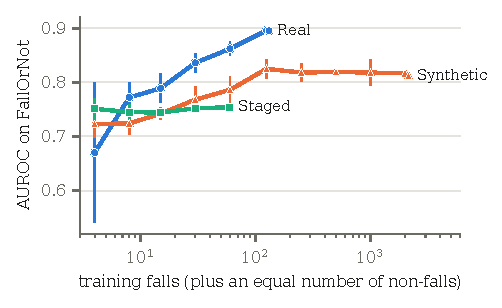
\includegraphics[width=\columnwidth]{fig_budget.pdf}
\caption{Equal training budget, CLIP + VideoMAE probes, FallOrNot test set (mean $\pm$ s.d.\ over random draws). Run 4.}
\label{fig:budget}
\end{figure}

\paragraph{Falls vs.\ other accidents.} Restricted to accident-moment clips (165 clips, 102 falls), CLIP + VideoMAE reaches 0.715 (staged), 0.772 (synthetic), 0.860 (real) and 0.848 (synthetic + real); zero-shot CLIP reaches 0.686. Telling a fall from another accident remains the hardest part of the task.

\subsection{On an independent source, the ranking flips}
On HMDB51 (\cref{tab:hmdb}, \cref{fig:flip}) the real-data advantage disappears. With CLIP + VideoMAE, real training is slightly \emph{worse} than synthetic ($-0.029$ [$-0.057$, $-0.003$], $p=0.029$) and no better than staged ($-0.011$, $p=0.57$). Synthetic training rescues VideoMAE ($+0.214$ over staged, $p<0.001$), and CLIP appearance trained on real OOPS!\ data falls to 0.626. HMDB51 falls look closer to staged falls than OOPS!\ accidents do: staged probes reach 0.899 there but 0.759 on FallOrNot, and zero-shot CLIP 0.834 vs.\ 0.717. Many HMDB51 falls come from films.

\begin{table}[t]\centering\small
\caption{AUROC on \textbf{HMDB51} (1,100 clips, 100 falls; nothing trained on it). Zero-shot CLIP: 0.834. Run 5.}
\label{tab:hmdb}
\begin{tabular}{lcccc}\toprule
Representation & Staged & Synthetic & Real & Syn.\ + real\\\midrule
CLIP appearance & 0.783 & \textbf{0.813} & 0.626 & 0.803\\
CLIP temporal & \textbf{0.887} & 0.866 & 0.825 & 0.842\\
VideoMAE & 0.664 & 0.877 & 0.779 & \textbf{0.901}\\
CLIP + VideoMAE & 0.899 & \textbf{0.917} & 0.888 & 0.901\\\midrule
\multicolumn{5}{l}{\footnotesize Hard subset (320 clips), CLIP + VideoMAE: staged 0.833, synthetic 0.880,}\\[-2pt]
\multicolumn{5}{l}{\footnotesize real 0.777, synthetic + real 0.855.}\\\bottomrule
\end{tabular}
\end{table}

\begin{figure}[t]\centering
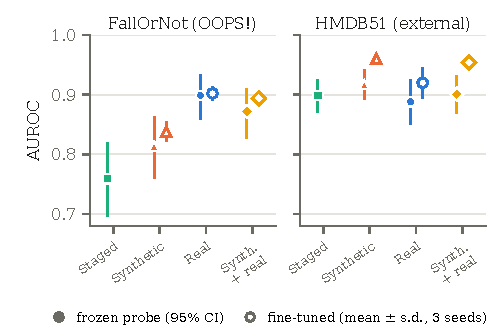
\includegraphics[width=\columnwidth]{fig_flip.pdf}
\caption{The ranking of training sources flips between real-world test sets. Filled: CLIP + VideoMAE probes with 95\% CIs (runs 4--5). Hollow: fine-tuned VideoMAE, mean $\pm$ s.d.\ over 3 seeds (run 7).}
\label{fig:flip}
\end{figure}

\subsection{Fine-tuning (pre-registered)}
The pre-registered test was \textbf{not met} for any of three seeds. On FallOrNot, fine-tuning on synthetic + real differs from the best probe by $-0.011$ to $-0.002$; on HMDB51 by $+0.028$ to $+0.049$ (CI above zero for two of three seeds). Averaged over seeds (\cref{tab:ft}), the flip reappears: real-trained models are best on FallOrNot and synthetic-trained models are best on HMDB51. Synthetic + real is within 0.008 of the best mean on both test sets and has the smallest seed-to-seed spread. Real-only fine-tuning varies strongly out of domain (HMDB51 hard subset 0.751--0.872).

\begin{table}[t]\centering\small
\caption{Fine-tuned VideoMAE, AUROC mean $\pm$ s.d.\ over 3 seeds. Runs 6--7.}
\label{tab:ft}
\begin{tabular}{lccc}\toprule
Trained on & FallOrNot & HMDB51 & HMDB51 hard\\\midrule
Synthetic & 0.838 $\pm$ 0.017 & \textbf{0.960 $\pm$ 0.006} & \textbf{0.922 $\pm$ 0.015}\\
Real & \textbf{0.902 $\pm$ 0.012} & 0.920 $\pm$ 0.026 & 0.795 $\pm$ 0.067\\
Synthetic + real & 0.894 $\pm$ 0.005 & 0.954 $\pm$ 0.011 & 0.890 $\pm$ 0.027\\\bottomrule
\end{tabular}
\end{table}

\subsection{Robustness to the annotator}\label{sec:annotator}
Re-grading FallOrNot with the second annotator's labels (99 videos, 152 clips, 78 falls; training labels unchanged) lowers absolute AUROC (best probe 0.797 instead of 0.899) but preserves the main findings: the staged-to-real gap; real over staged training ($+0.083$ [$+0.010$, $+0.157$], $p=0.024$; CLIP temporal $+0.100$, $p=0.010$); the learning-curve shape (about 8 real falls match staged training, 15 exceed it); and the synthetic plateau below real data at equal budget. The in-domain advantage of real over synthetic training shrinks to $+0.065$ [$-0.006$, $+0.137$] and is no longer significant ($p=0.079$).

%=====================================================================
\section{Discussion}
\paragraph{Which data should a practitioner collect?} In the domain where real falls are collected, a few dozen of them are worth more than thousands of synthetic falls. But that advantage does not travel: on another real-world source, synthetic data generalised better. Mixing synthetic and real data was the only recipe near the top on both test sets, for both frozen probes and fine-tuned models.

\paragraph{One real-world benchmark is not enough.} The ranking of training sources reversed between FallOrNot and HMDB51, and the two benchmarks disagree even about how hard real falls are (staged probes: 0.759 vs.\ 0.899). Claims such as ``synthetic beats staged'' or ``real beats synthetic'' should be tested on more than one in-the-wild source.

\paragraph{False alarms on other accidents.} Most fall benchmarks contain falls and everyday activities. FallOrNot's accident negatives show that separating a fall from a collision or a near-fall is the hardest sub-problem, and should be part of evaluation.

%=====================================================================
\section{Limitations}
\begin{itemize}\setlength\itemsep{1pt}
\item \textbf{Label uncertainty.} Agreement between annotators was moderate ($\kappa=0.50$), and absolute scores depend on the annotator; the fall definition needs sharper written guidance.
\item \textbf{Scale.} 165 labelled test videos and 268 real training clips; confidence intervals are wide.
\item \textbf{In-domain real data.} Real training and test clips both come from OOPS!; the real-data advantage on FallOrNot is partly in-domain advantage.
\item \textbf{Imperfect external test.} HMDB51 falls are partly from films and trimmed to the action; they are real-world video but not necessarily real accidents.
\item \textbf{Population.} Neither source focuses on older adults at home, the main use case.
\item \textbf{One staged dataset} (UR Fall), which is saturated in-domain.
\item \textbf{Model-selected training pool.} The real training clips were pre-selected by a CLIP zero-shot score; the test sample was not.
\item \textbf{Fixed fine-tuning hyper-parameters} were not tuned; three seeds only.
\end{itemize}

\section{Conclusion}
Staged-trained fall detectors that look perfect in the lab fail on real accidents. On the source where real falls are collected, a few dozen of them outperform thousands of synthetic falls, but on an independent real-world source the ranking flips. Training on synthetic and real data together is the most robust choice we found, and fall detection should be evaluated on more than one real-world source. We release FallOrNot's labels, timestamps and code.

\paragraph{Data and ethics.} OOPS!\ videos are public web videos; we release only labels, timestamps and code. UR Fall is licensed CC BY-NC-SA 4.0 for non-commercial research; HMDB51 is CC BY 4.0; OmniFall annotations are released for non-commercial use.

%=====================================================================
\small
\begin{thebibliography}{99}
\bibitem{auvinet_mcfd} E.~Auvinet, C.~Rougier, J.~Meunier, A.~St-Arnaud, and J.~Rousseau. Multiple cameras fall data set. Technical Report 1350, DIRO, Universit\'e de Montr\'eal, 2010.
\bibitem{bagala2012} F.~Bagal\`a et~al. Evaluation of accelerometer-based fall detection algorithms on real-world falls. \emph{PLoS ONE}, 7(5):e37062, 2012.
\bibitem{charfi2013} I.~Charfi, J.~Miteran, J.~Dubois, M.~Atri, and R.~Tourki. Optimized spatio-temporal descriptors for real-time fall detection: comparison of support vector machine and Adaboost-based classification. \emph{Journal of Electronic Imaging}, 22(4):041106, 2013.
\bibitem{epstein2020oops} D.~Epstein, B.~Chen, and C.~Vondrick. Oops! Predicting unintentional action in video. In \emph{CVPR}, 2020.
\bibitem{fleming2008} J.~Fleming and C.~Brayne. Inability to get up after falling, subsequent time on floor, and summoning help: prospective cohort study in people over 90. \emph{BMJ}, 337:a2227, 2008.
\bibitem{gadre2023datacomp} S.~Y. Gadre et~al. DataComp: In search of the next generation of multimodal datasets. In \emph{NeurIPS Datasets and Benchmarks Track}, 2023.
\bibitem{kay2017kinetics} W.~Kay et~al. The Kinetics human action video dataset. arXiv:1705.06950, 2017.
\bibitem{klenk2016} J.~Klenk et~al. The FARSEEING real-world fall repository: a large-scale collaborative database to collect and share sensor signals from real-world falls. \emph{European Review of Aging and Physical Activity}, 13:8, 2016.
\bibitem{kuehne2011hmdb} H.~Kuehne, H.~Jhuang, E.~Garrote, T.~Poggio, and T.~Serre. HMDB: A large video database for human motion recognition. In \emph{ICCV}, pages 2556--2563, 2011.
\bibitem{kwolek2014} B.~Kwolek and M.~Kepski. Human fall detection on embedded platform using depth maps and wireless accelerometer. \emph{Computer Methods and Programs in Biomedicine}, 117(3):489--501, 2014.
\bibitem{omnifall} D.~Schneider et~al. OmniFall: From staged through synthetic to wild, a unified multi-domain dataset for robust fall detection. arXiv:2505.19889, 2025 (v3, 2026).
\bibitem{openclip} G.~Ilharco, M.~Wortsman, R.~Wightman, C.~Gordon, N.~Carlini, R.~Taori, A.~Dave, V.~Shankar, H.~Namkoong, J.~Miller, H.~Hajishirzi, A.~Farhadi, and L.~Schmidt. OpenCLIP. Zenodo, 2021. doi:10.5281/zenodo.5143773.
\bibitem{radford2021clip} A.~Radford et~al. Learning transferable visual models from natural language supervision. In \emph{ICML}, 2021.
\bibitem{tong2022videomae} Z.~Tong, Y.~Song, J.~Wang, and L.~Wang. VideoMAE: Masked autoencoders are data-efficient learners for self-supervised video pre-training. In \emph{NeurIPS}, 2022.
\bibitem{who_falls} World Health Organization. Falls (fact sheet), 21 October 2026. \url{https://www.who.int/news-room/fact-sheets/detail/falls}, accessed November 2026.
\end{thebibliography}
\end{document}
